This paper seeks to determine the best-performing neural network for tool image classification. The best-performing neural network is determined in the course of an experiment. The experiment is conducted by training and evaluating selected neural networks on a dataset. The Dataset, selected neural networks, training, and evaluation are described in this chapter. To measure performance, accuracy is used, see Section \ref{sec:metric}. The results of this experiment are reported in Chapter~\ref{chp:result}. To conduct the experiment, Movilizer GmbH provided $200$ hours on an Amazon Web Service g4dn.xlarge instance running a Deep Learning AMI (Ubuntu 18.04).\autocite{AWS.2020a}
The g4dn.xlarge instance provides 4 vCPUs, 16GB RAM, 125GB storage, and a NVIDIA~T4~GPU. \autocite{AWS.2020b} 
The experiment is implemented in Python 3\autocite{Python3} using Keras~2.2.4.2\autocite{Keras}, Tensorflow 2.1.0\autocite{Tensorflow.2015}, CUDA 10.1\autocite{CUDA}, and cuDNN\autocite{cuDNN}. The dataset and code used to conduct the experiment are appended in the digital appendix, see Section \ref{sec:digiappend}.

\subsection{Dataset}
The dataset is constructed as described in Section \ref{sec:datasetconstruction}. The constructed dataset is comprised of tool images for image classification. Therefore, it is named \ac{TIC Dataset}. The \ac{TIC Dataset} is comprised of $20{,}400$ tool images of six classes. The classes are listed below.
\begin{itemize}
	\item drill
	\item hammer
	\item pliers
	\item saw
	\item screwdriver
	\item wrench
\end{itemize}
Each class comprises $3{,}400$ tool images. A tool image is a close-up image of exactly one tool. 
For a class, tool images display different tools of the same class from arbitrary angles and with arbitrary backgrounds. Figure \ref{fig:screwdriver} illustrates this for the class screwdriver with two images of different tools.
\begin{figure}[H]
	\centering
	\begin{subfigure}[b]{0.45\textwidth}
		\centering
		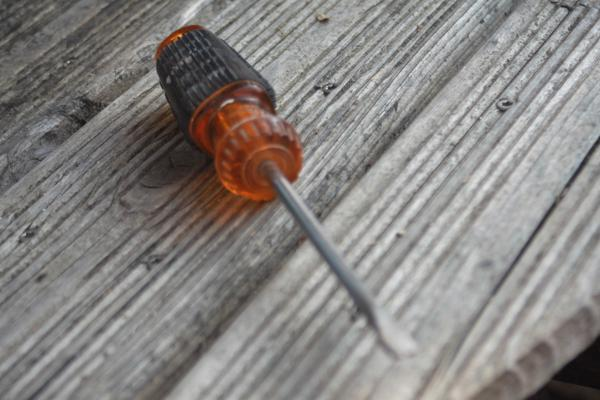
\includegraphics[width=\textwidth]{img/screwdriver1}
	\end{subfigure}
	\hfill
	\begin{subfigure}[b]{0.45\textwidth}
		\centering
		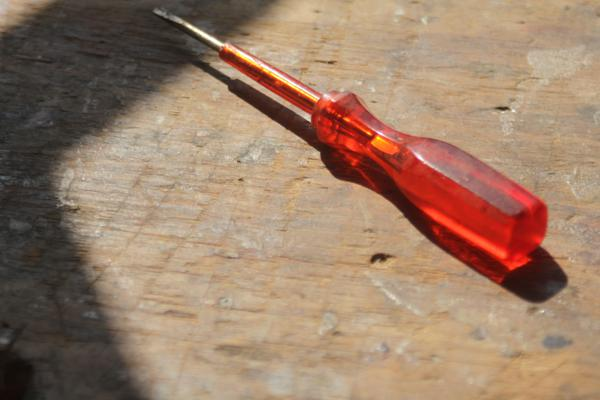
\includegraphics[width=\textwidth]{img/screwdriver2}
	\end{subfigure}
	\caption{Two Images from the TIC Dataset of Class Screwdriver (own figure)}
	\label{fig:screwdriver}
\end{figure}
The dataset is split into a training, validation, and test dataset. For each class, $60\%$ of the images are randomly split for the training dataset, $20\%$ for the validation dataset, and $20\%$ for the test dataset. The resulting training dataset contains $12{,}240$, the resulting validation dataset contains $4{,}080$, and the resulting test dataset contains $4{,}080$ images. For each of these datasets, the images are evenly distributed over all classes.
The training dataset is used to train a neural network. The validation dataset and the test dataset are not used for training. On that account, the neural network cannot overfit to the validation dataset and the test dataset. Thus, the validation dataset can be used to explore different hyperparameters and monitor whether or not the neural network overfits to the training dataset. Based on the performance on the validation dataset, the neural network is chosen for evaluation. This way, the neural network might develop a dependency on the validation dataset. For example, a neural network might perform well on the validation dataset by chance but less well on other data. For this reason, the neural network is evaluated only once on the test dataset. The performance of  the neural network on the test dataset is regarded as the performance of the neural network. \autocite{ElAmir.2020}



\subsection{Neural Network Selection}
To determine the best-performing neural network for tool image classification, optimally, this paper would conduct a neural network architecture search and hyperparameter search. However, resources and time of this paper are limited. Due to that, conducting a neural network architecture search and hyperparameter search is not possible. 
\par
Tool image classification is a sub-task of image classification. Therefore, this paper selects the state-of-the-art neural networks for image classification to conduct the experiment. The state-of-the-art neural networks for image classification are determined as described in Section \ref{sec:litrev}. For each selected neural network the network architecture and the hyperparameters are adopted from the paper originally proposing the neural network. The following neural networks are selected to conduct the experiment:
\begin{itemize}
	\item VGG-19, see Section \ref{sec:conv}. \autocite{Simonyan.2014}
	\item ResNet-152, see Section \ref{sec:res}. \autocite{He.2016}
	\item ResNext-101, see Section \ref{sec:inception}. \autocite{Xie.2017}
	\item DenseNet-264, see Section \ref{sec:dense}. \autocite{Huang.2017}
	\item EfficientNet-B7, see Section \ref{sec:sepconv}. \autocite{Tan.2019}
\end{itemize}
This paper implements the selected neural networks based on their Keras implementation.\autocite{KerasApp} Note that CapsNet is excluded since it does not reach state-of-the-art performance on image classification except for classification of digits or letters.



\subsection{Training}% Training Hyperparams
The neural networks are trained on the training dataset and their performance is monitored on the validation dataset.
Training is carried out by optimizing the categorical cross entropy loss function \autocites{Michelucci.2019}{ElAmir.2020}{Singh.2020}, see Section \ref{sec:training}. Each selected neural network is trained with the number of epochs, the optimizer, and the hyperparameters of the optimizer as specified in the paper originally proposing the neural network.
The hyperparameters of the optimizer are initial learning rate, learning rate schedule, and momentum or Nesterove momentum if used. The learning rate schedule determines how the learning rate changes with epochs progressing.
The batch size specified in the original papers are powers of 2. However, those batch sizes are too large to fit the available GPU. Therefore, the power is reduced by one until the batch size fits the available GPU. For each neural network, the training hyperparameters, namely number of epochs, the optimizer, the hyperparameters of the optimizer, and the batch size are displayed in Table \ref{tab:hyperparams}. \autocites{Simonyan.2014}{He.2016}{Xie.2017}{Huang.2017}{Tan.2019}
\par
For EfficientNet-B7, the number of epochs is not specified, instead EfficientNet-B7 is trained until convergence. \autocite{Tan.2019} The available $200$ hours on the provided hardware might not be enough to train EfficientNet-B7 until convergence. Therefore, the other neural networks are trained before EfficientNet-B7. EfficientNet-B7 is trained for the remaining time.
\begin{xltabular}{\textwidth}{llX}\toprule
	\caption[Training Hyperparameters]{Training Hyperparameters \autocites{Simonyan.2014}{He.2016}{Xie.2017}{Huang.2017}{Tan.2019}} \label{tab:hyperparams}\\
	\textbf{Neural Network} & \textbf{Training Hyperparameters} & \\\midrule \endhead
	VGG-19 & Epochs: & $74$\\
		& Optimizer: & \ac{SGD}\\
		& Initial Learning Rate: & $0.01$\\
		& Learning Rate Schedule: & divide learning rate by $10$ on accuracy plateaus.\\
		& Momentum: & $0.9$\\
		& Batch Size: & $32$\\
	\\\midrule
	ResNet-152 & Epochs: & $120$\\
		& Optimizer: & \ac{SGD}\\
		& Initial Learning Rate: & $0.1$\\
		& Learning Rate Schedule: & divide learning rate by $10$ on accuracy plateaus.\\
		& Momentum: & $0.9$\\ 
		& Batch Size: & $32$\\
	\\\midrule
	ResNeXt-101 & Epochs: & $120$\\
		& Optimizer: & \ac{SGD}\\
		& Initial Learning Rate: & $0.1$\\
		& Learning Rate Schedule: & divide learning rate by $10$ at epoch $30$, $60$, and $90$.\\
		& Momentum: & $0.9$\\ 
		& Batch Size: & $16$\\
	\\\midrule
	DenseNet-264 & Epochs: & $90$\\
		& Optimizer: & \ac{SGD}\\
		& Initial Learning Rate: & $0.1$\\
		& Learning Rate Schedule: & divide learning rate by $10$ at epoch $30$ and $60$.\\
		& Nesterov Momentum: & $0.9$\\
		& Batch Size: & $32$\\
	\\\midrule
	EfficientNet-B7 & Epochs: & not specified\\
		& Optimizer: & \ac{RMSProp}\\
		& Initial Learning Rate: & $0.256$\\
		& Learning Rate Schedule: & decay learning rate by $0.97$ each $2.4$ epochs.\\
		& Momentum: & $0.9$\\
		& Batch Size: & $1$
	\\\bottomrule
\end{xltabular}
Note that metalearning, semi- or unsupervised learning, transfer learning, adversarial training, data augmentation, input normalization, weight decay, and multi-task learning are excluded from the scope of this paper,  see Section \ref{sec:scope}. In consequence, they are excluded from the experiment even if they are used in the original papers.

\subsection{Evaluation}
As mentioned, during training the performance of each neural network is monitored on the validation dataset. The performance is measured at the end of each epoch. After training for the entire number of epochs, the neural network from the epoch with the highest performance is evaluated. A neural network is evaluated on the test dataset. The resulting performance measured in accuracy is reported in Chapter \ref{chp:result}.
